\documentclass[english]{article}
\usepackage[T1]{fontenc}
\usepackage[latin9]{inputenc}
\usepackage{babel}
\usepackage{graphicx}
\usepackage{subfigure}
\usepackage{float}
\setlength{\parindent}{0pt}
\usepackage{amsmath}


\begin{document}

\title{Lab 4: Compact Vision System\\ -------------------------------- \\ \Large Sensors and Digitization}
\author{ \ Armine Vardazaryan, Songyou Peng \\ arminevardazaryan@gmail.com, psy920710@gmail.com}
\date{9rd December 2015}

\maketitle

\section{Introduction}
In this laboratory work we used the KEYENCE CV-020
machine vision system to measure and identify objects. In the first part of the lab work we measured the edge pitch of some industrial parts. 
And in the second part, we setup the smart system to recognize objects in its field of view.
\section{Edge Detection}
In the first part of the laboratory work, we used the provided system to measure the size of an object.
In particular, we wanted to measure the width of the holders of the shown objects.\\
\begin{figure}[H]
	\centering
	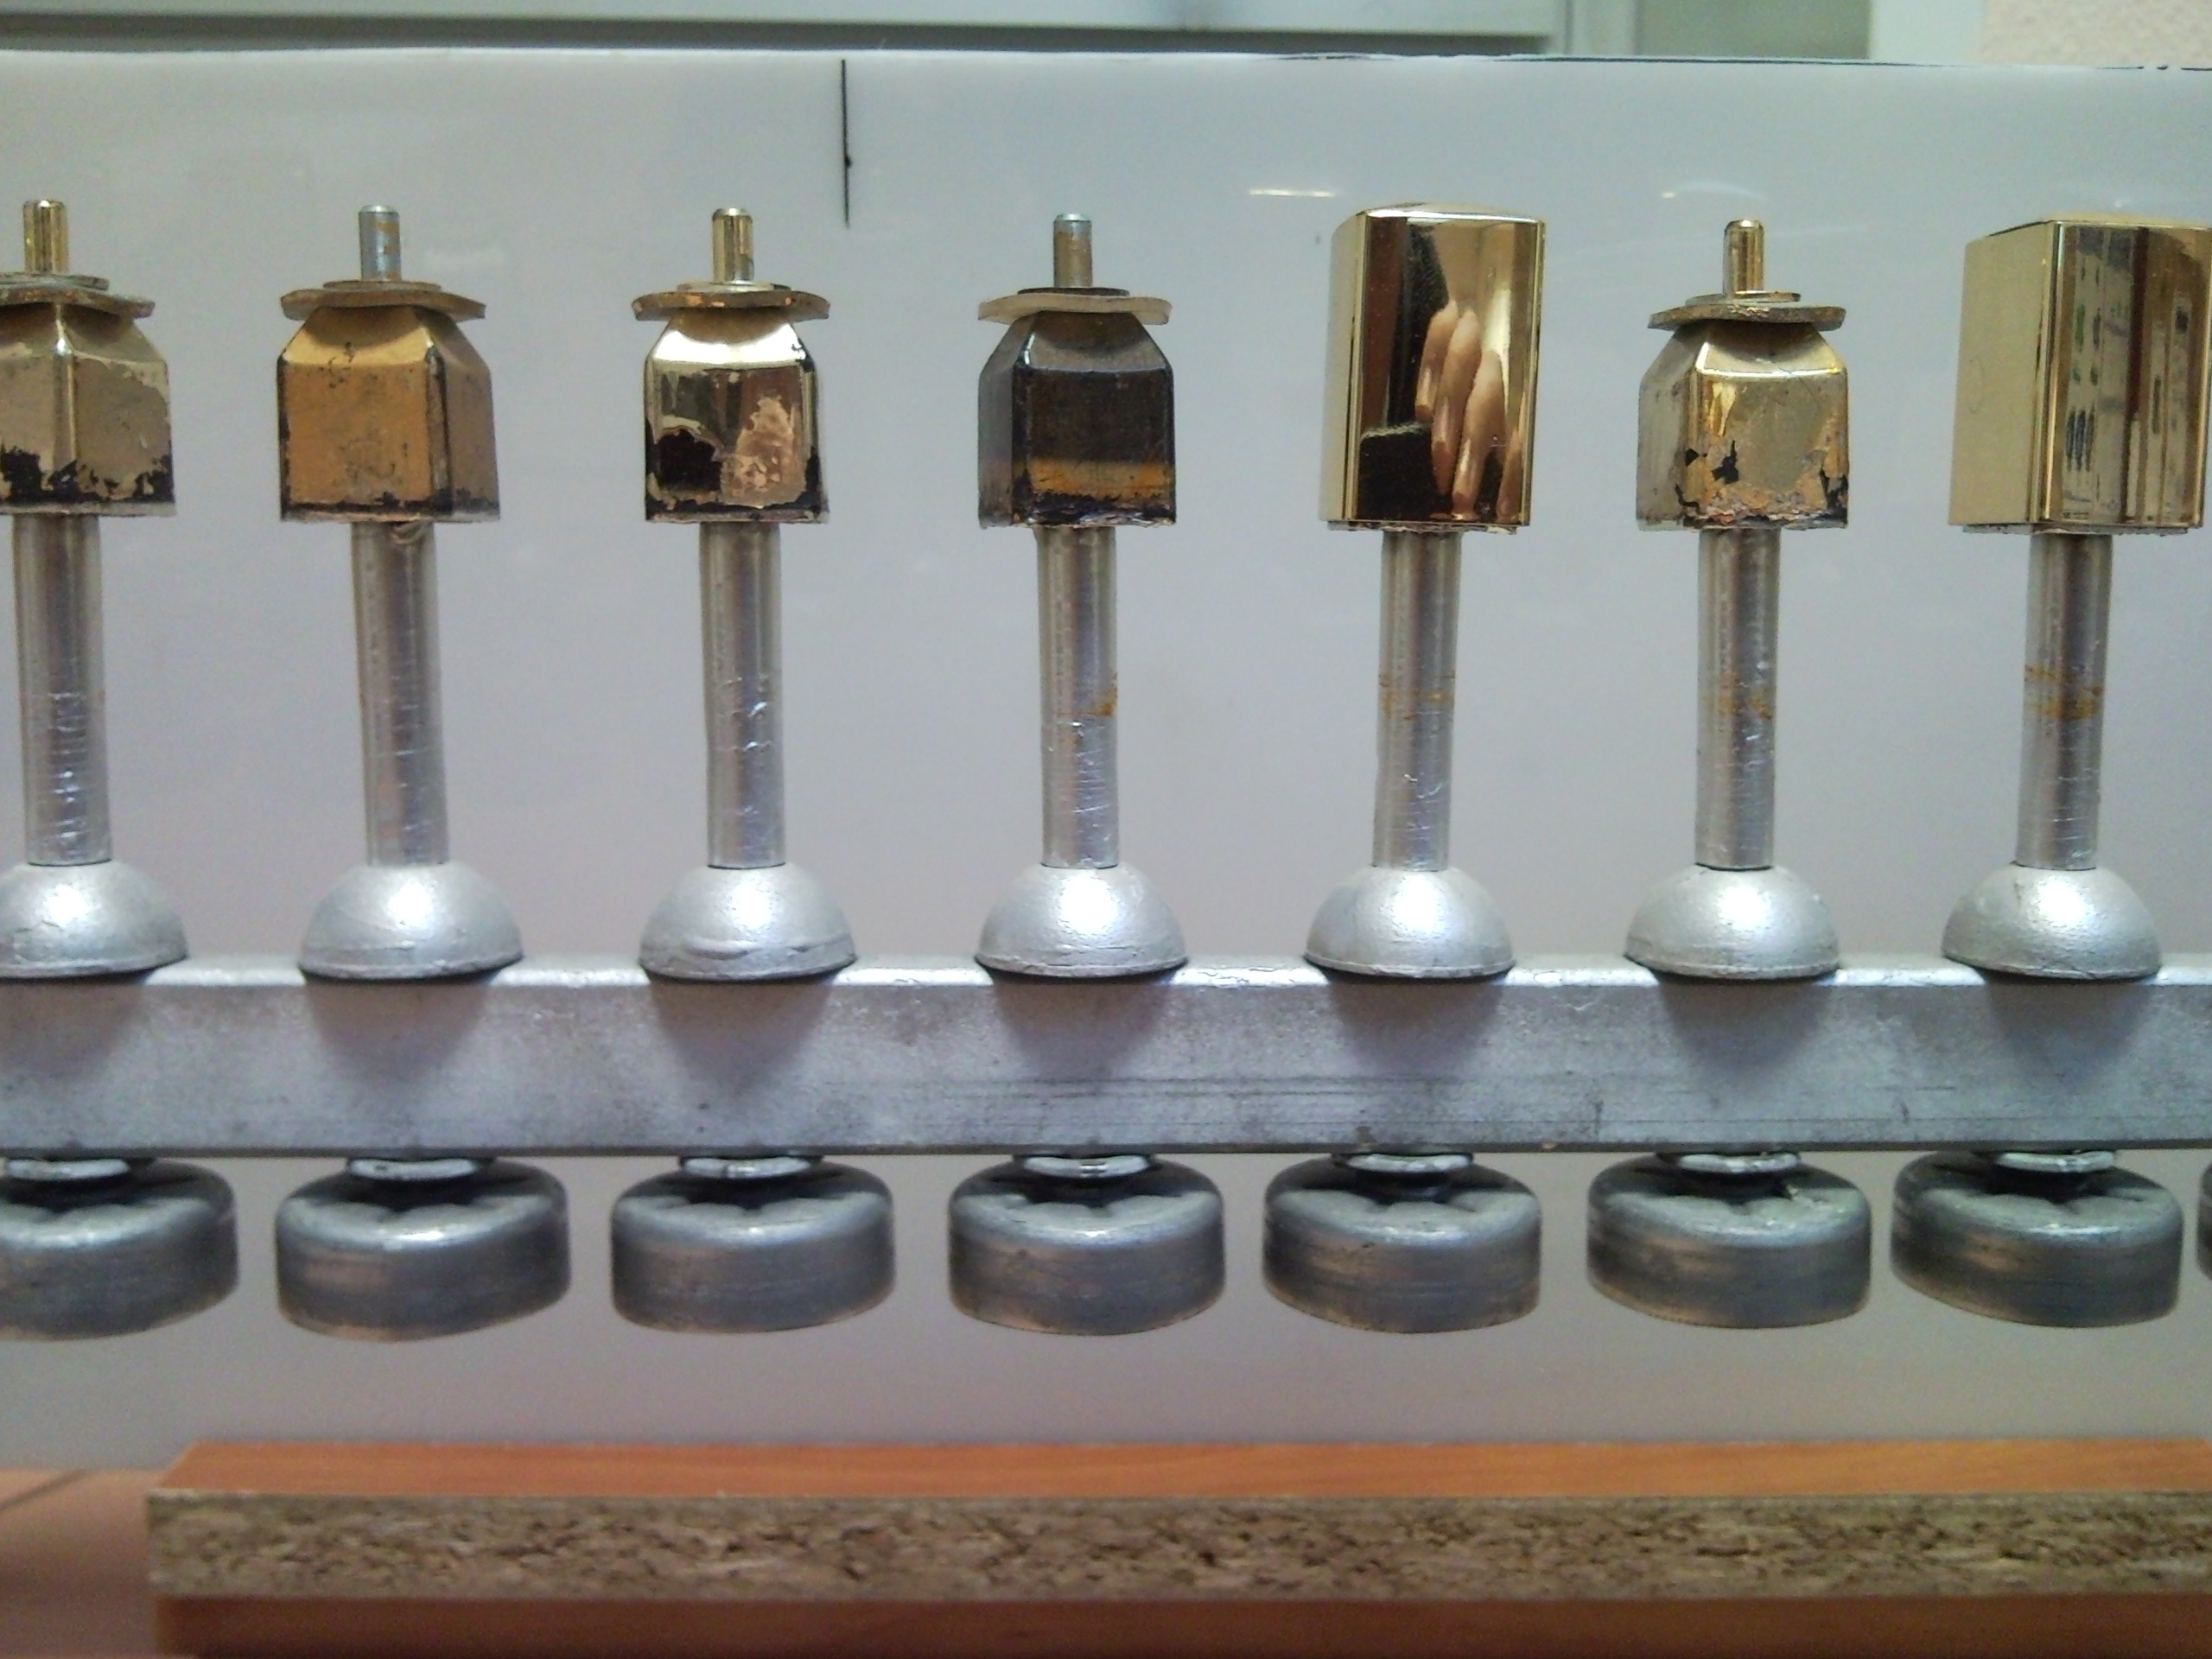
\includegraphics[width=0.45\linewidth]{Pictures/SNC00006.jpg}
	\caption{The objects that we want to measure}
	\label{fig:origobj}
\end{figure} 
To measure the sizes of the holders, we used the KEYENCE embedded software.
To setup this kind of measurement, first, we create a new program, then navigate to a menu item "Window Settings", where we choose Edge pitch as the type of the measurement.
Then we create a measure window in the same section.
The measurement window is the area where the edges will be looked for. The measurement window is as follows.
\begin{figure}[H]
	\centering
	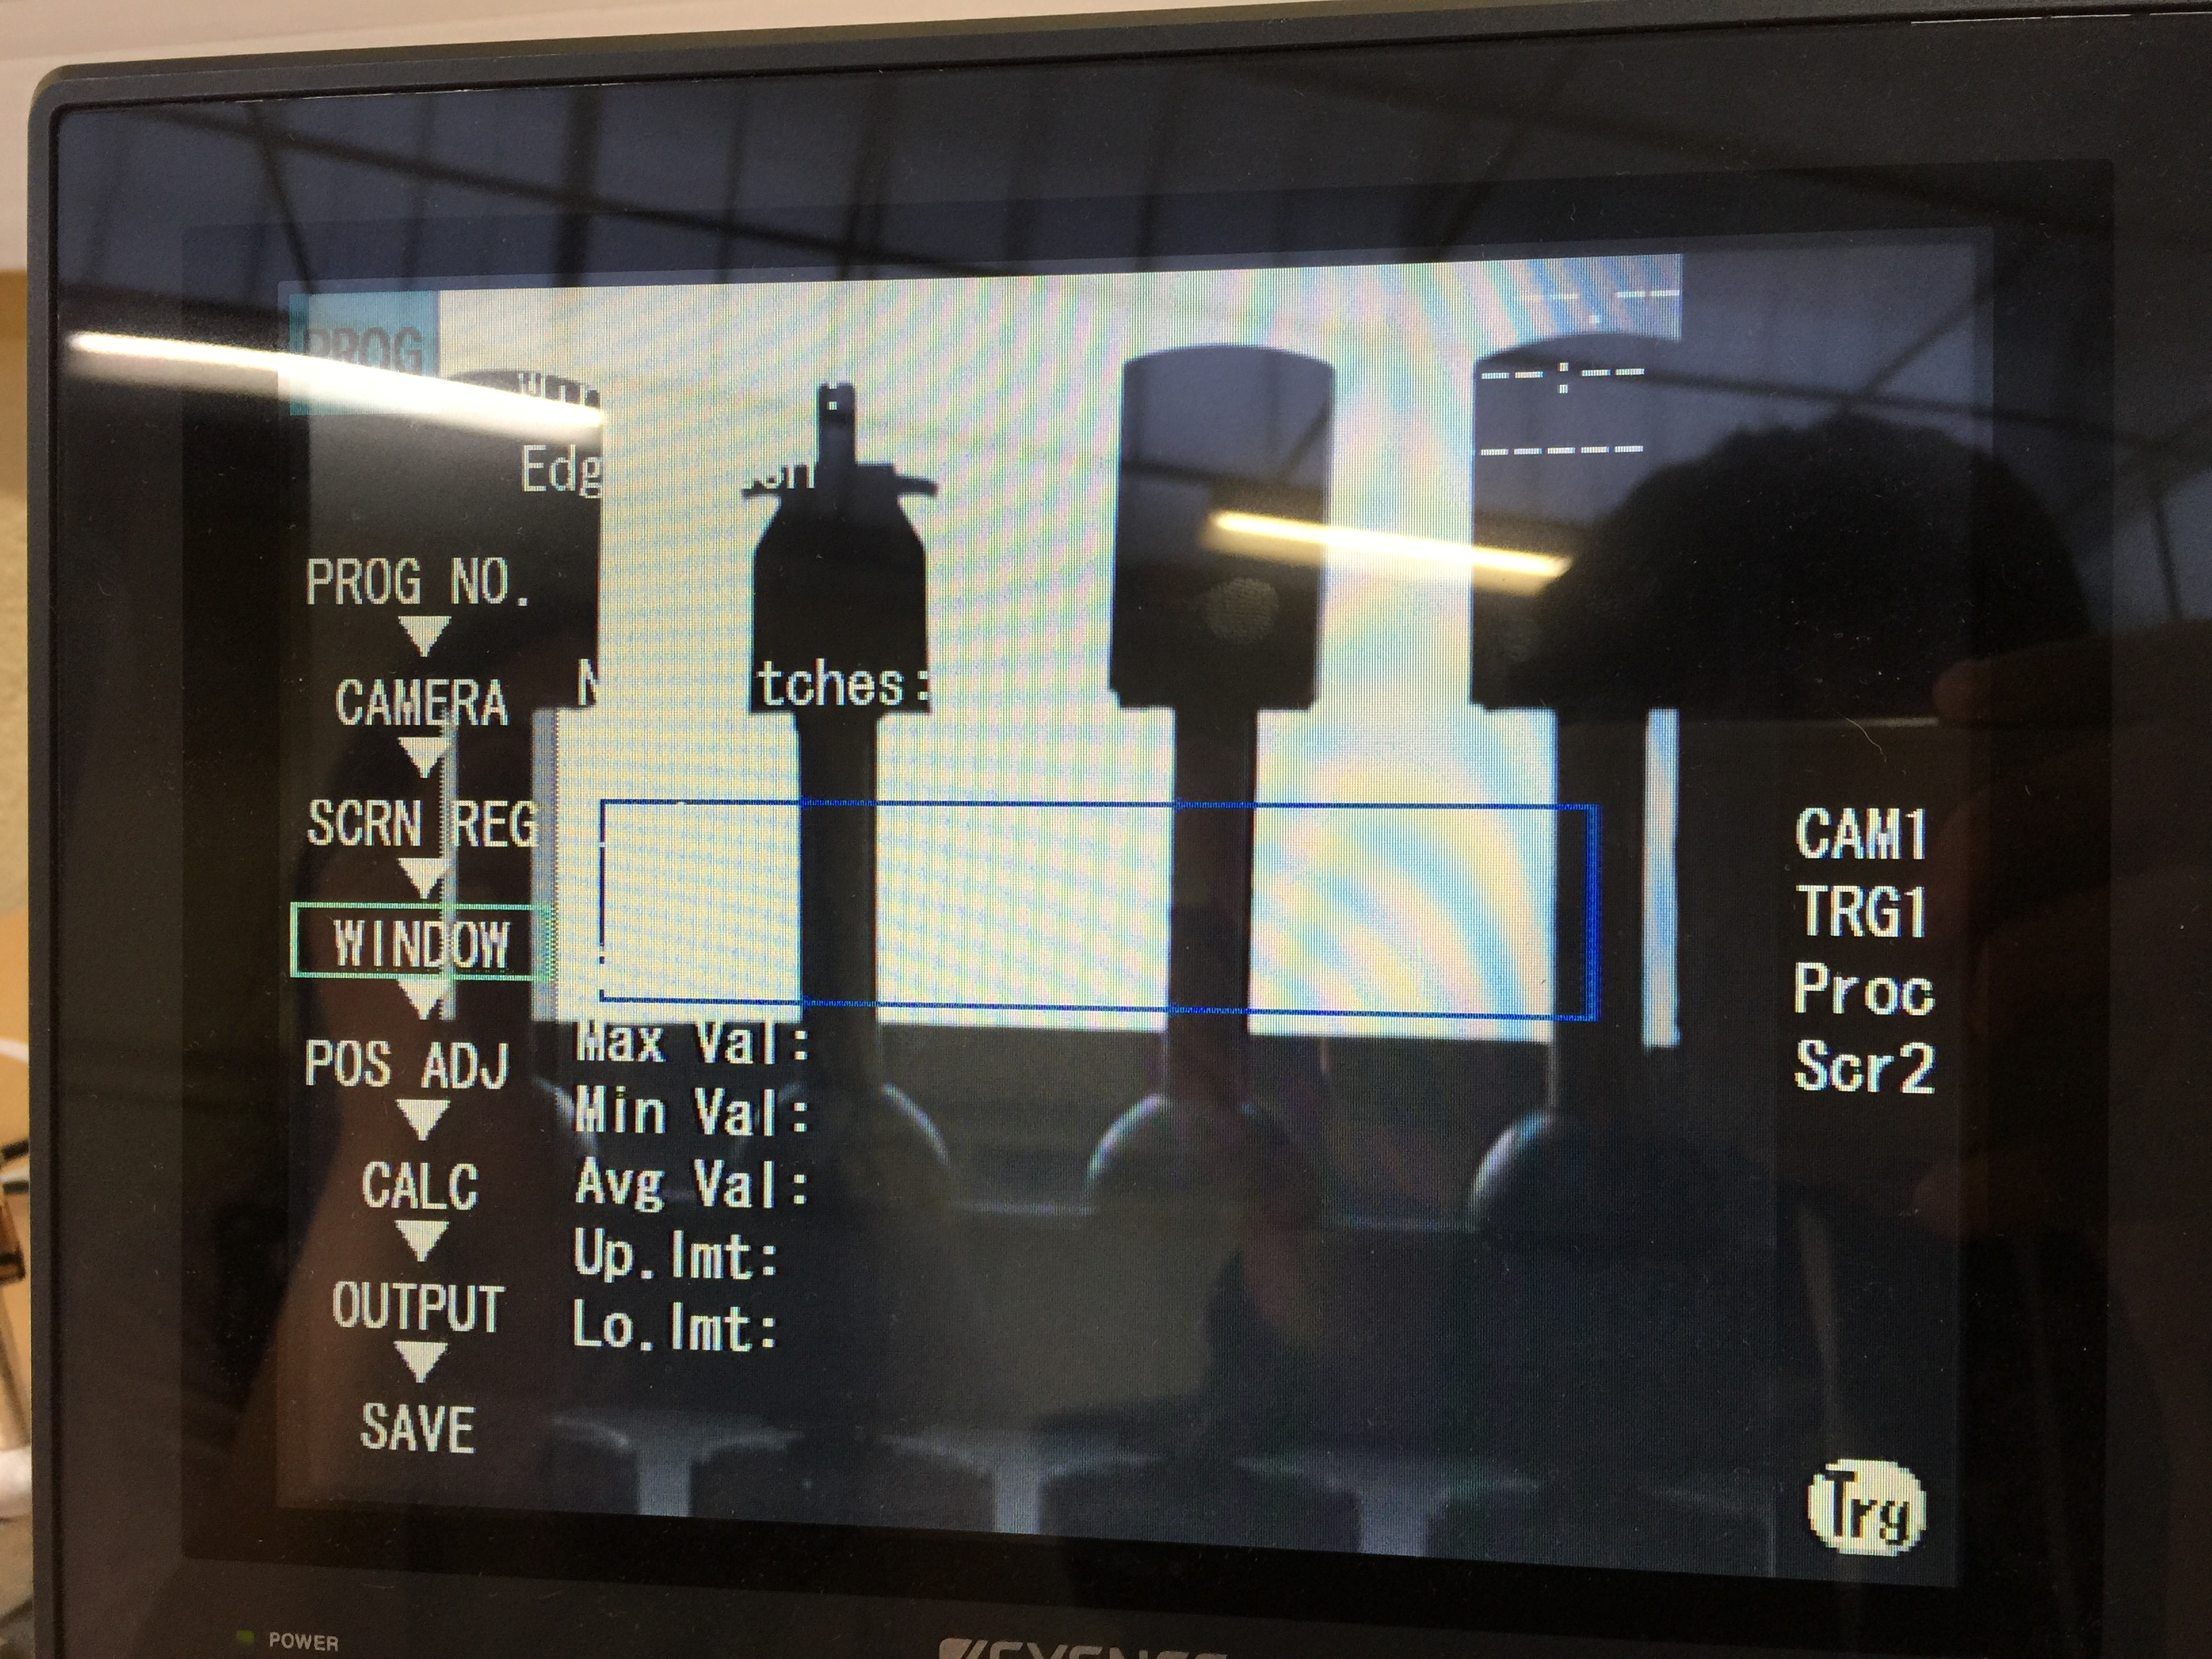
\includegraphics[width=0.6\linewidth]{Pictures/IMG_1221.JPG}
	\caption{The measurement area outlined with blue}
	\label{fig:measwind}
\end{figure} 

After completing the settings, we executed the program.

\begin{figure}[H]
	\centering
	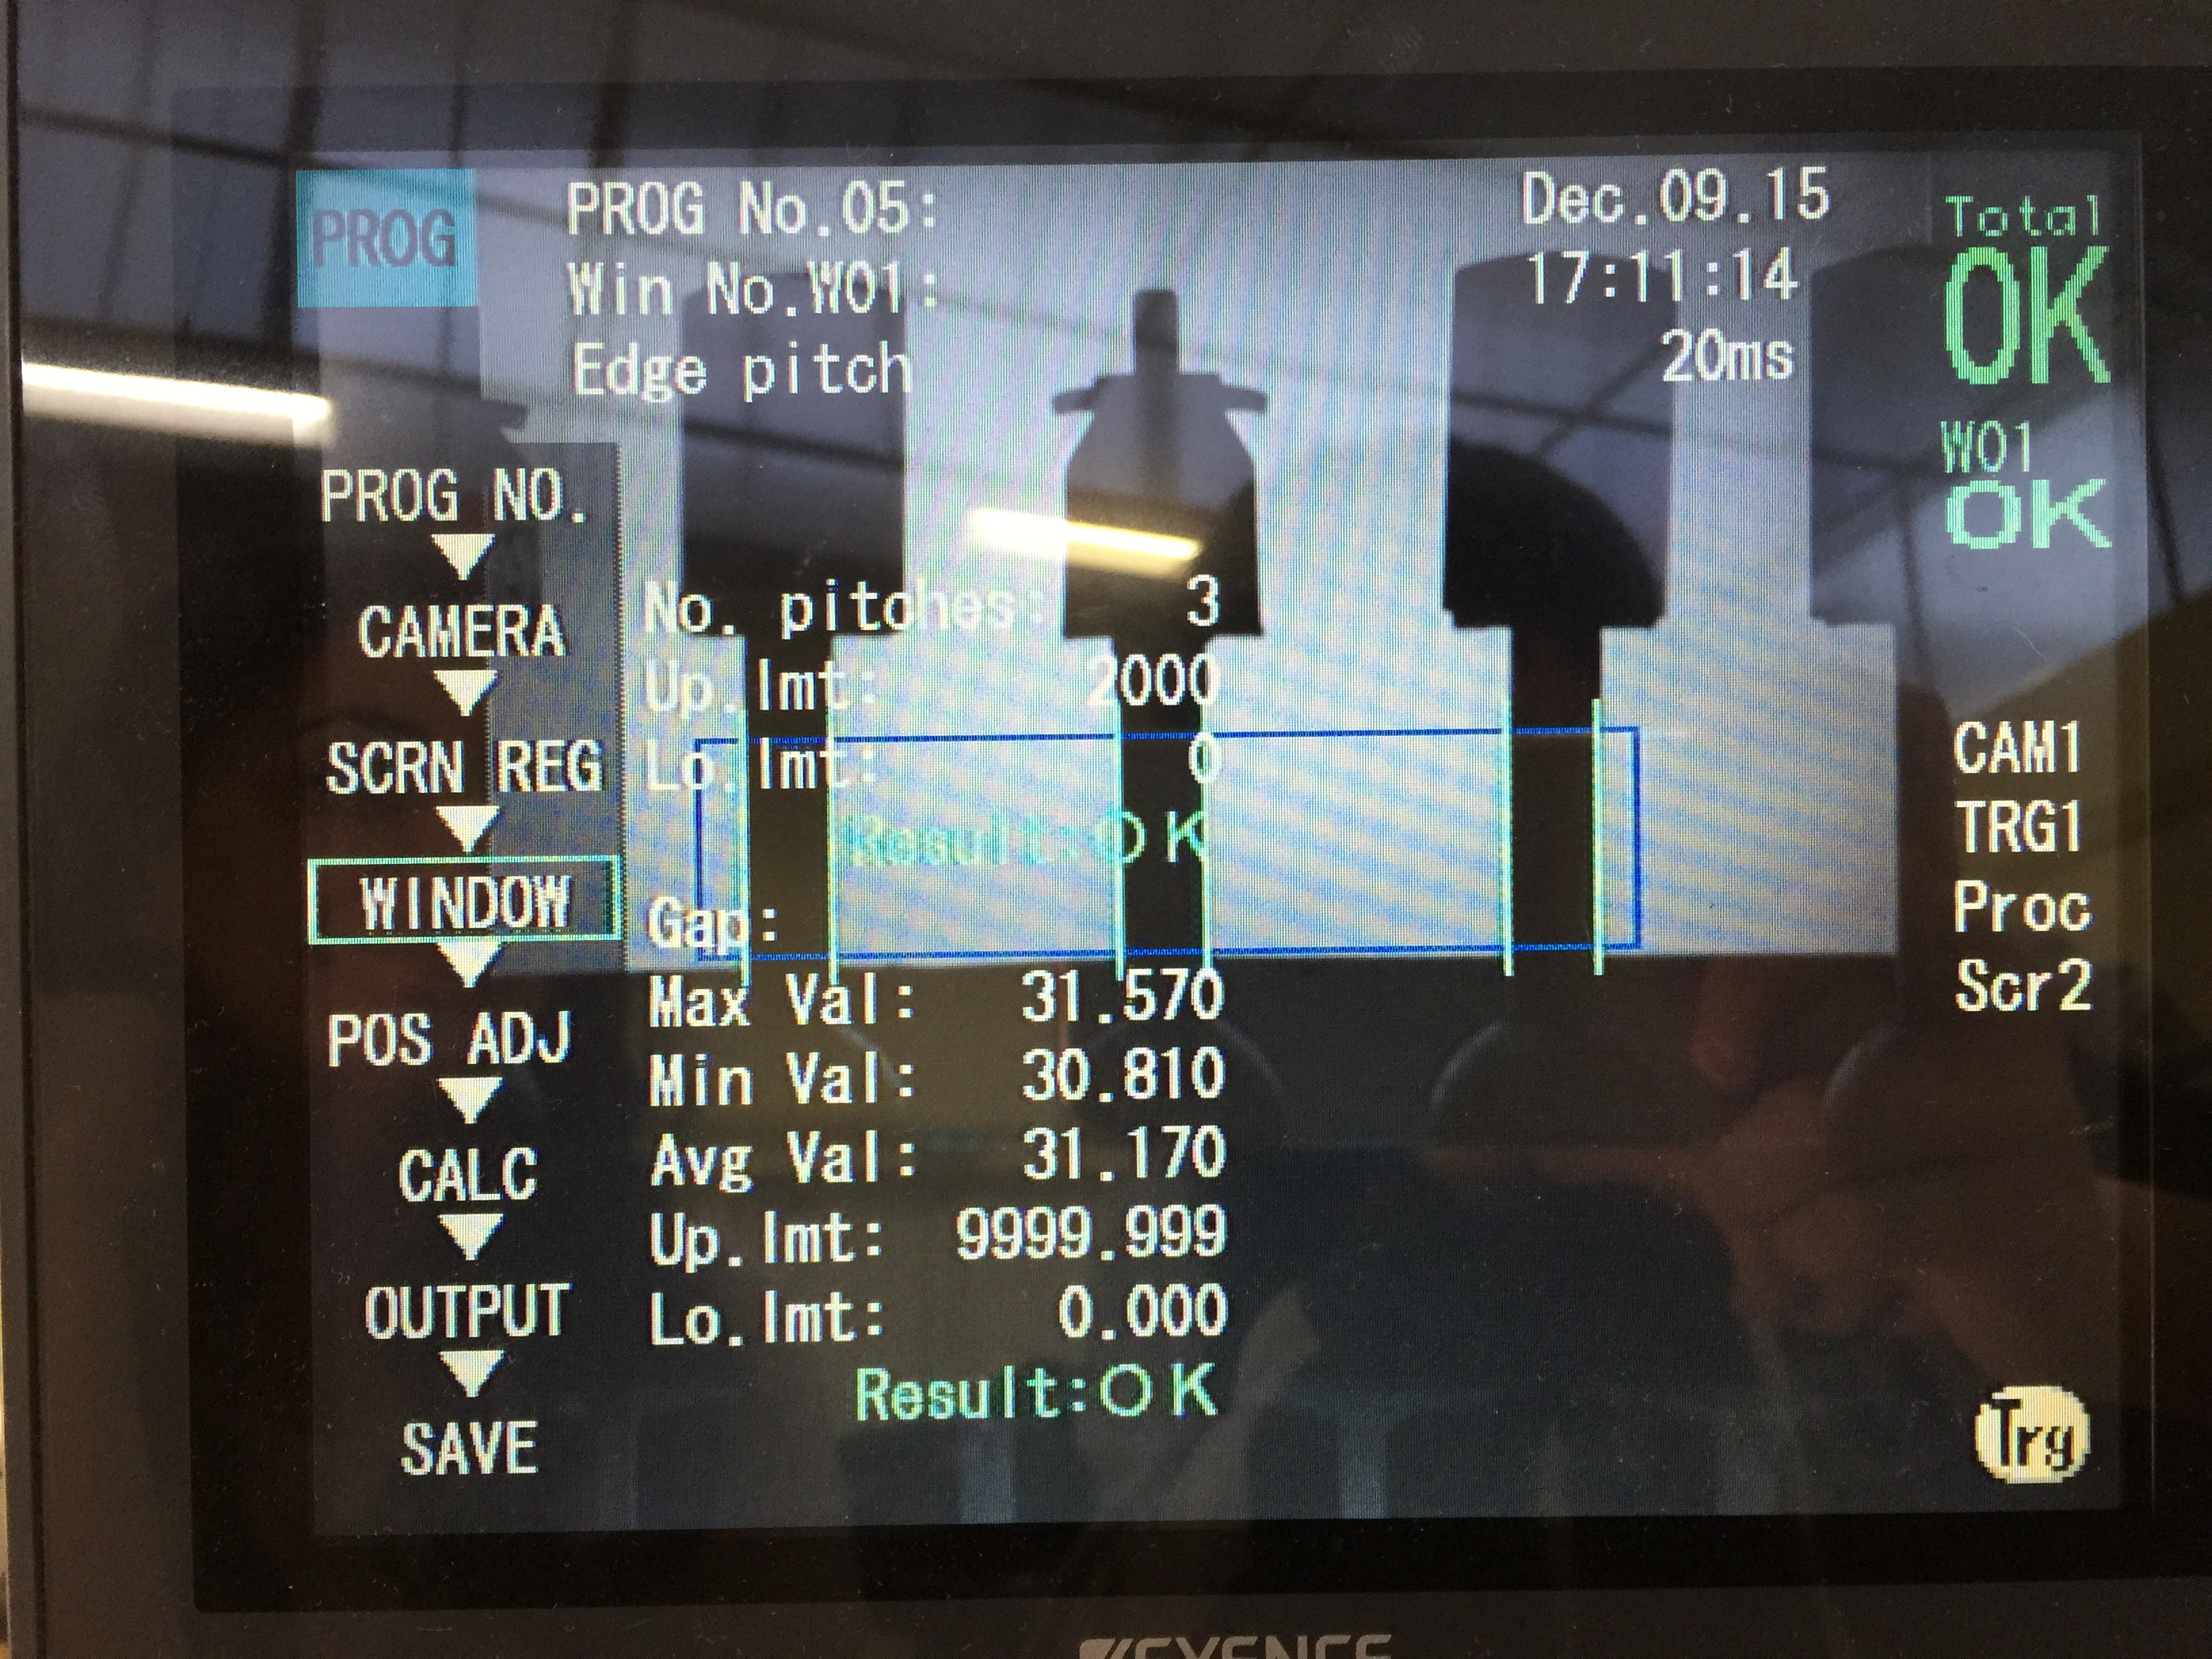
\includegraphics[width=0.6\linewidth]{Pictures/IMG_1222.JPG}
	\caption{Measurement of edge pitch}
	\label{fig:edgepitch}
\end{figure} 
In \ref{fig:edgepitch} we see that the program is able to identify and measure the edge widths of the objects.
As three of them are located in the measurement area, number of pitches is 3, and the average measured value is 31.17.
A second try, this time with two of the objects in the field of measurement yielded the following result.
\begin{figure}[H]
	\centering
	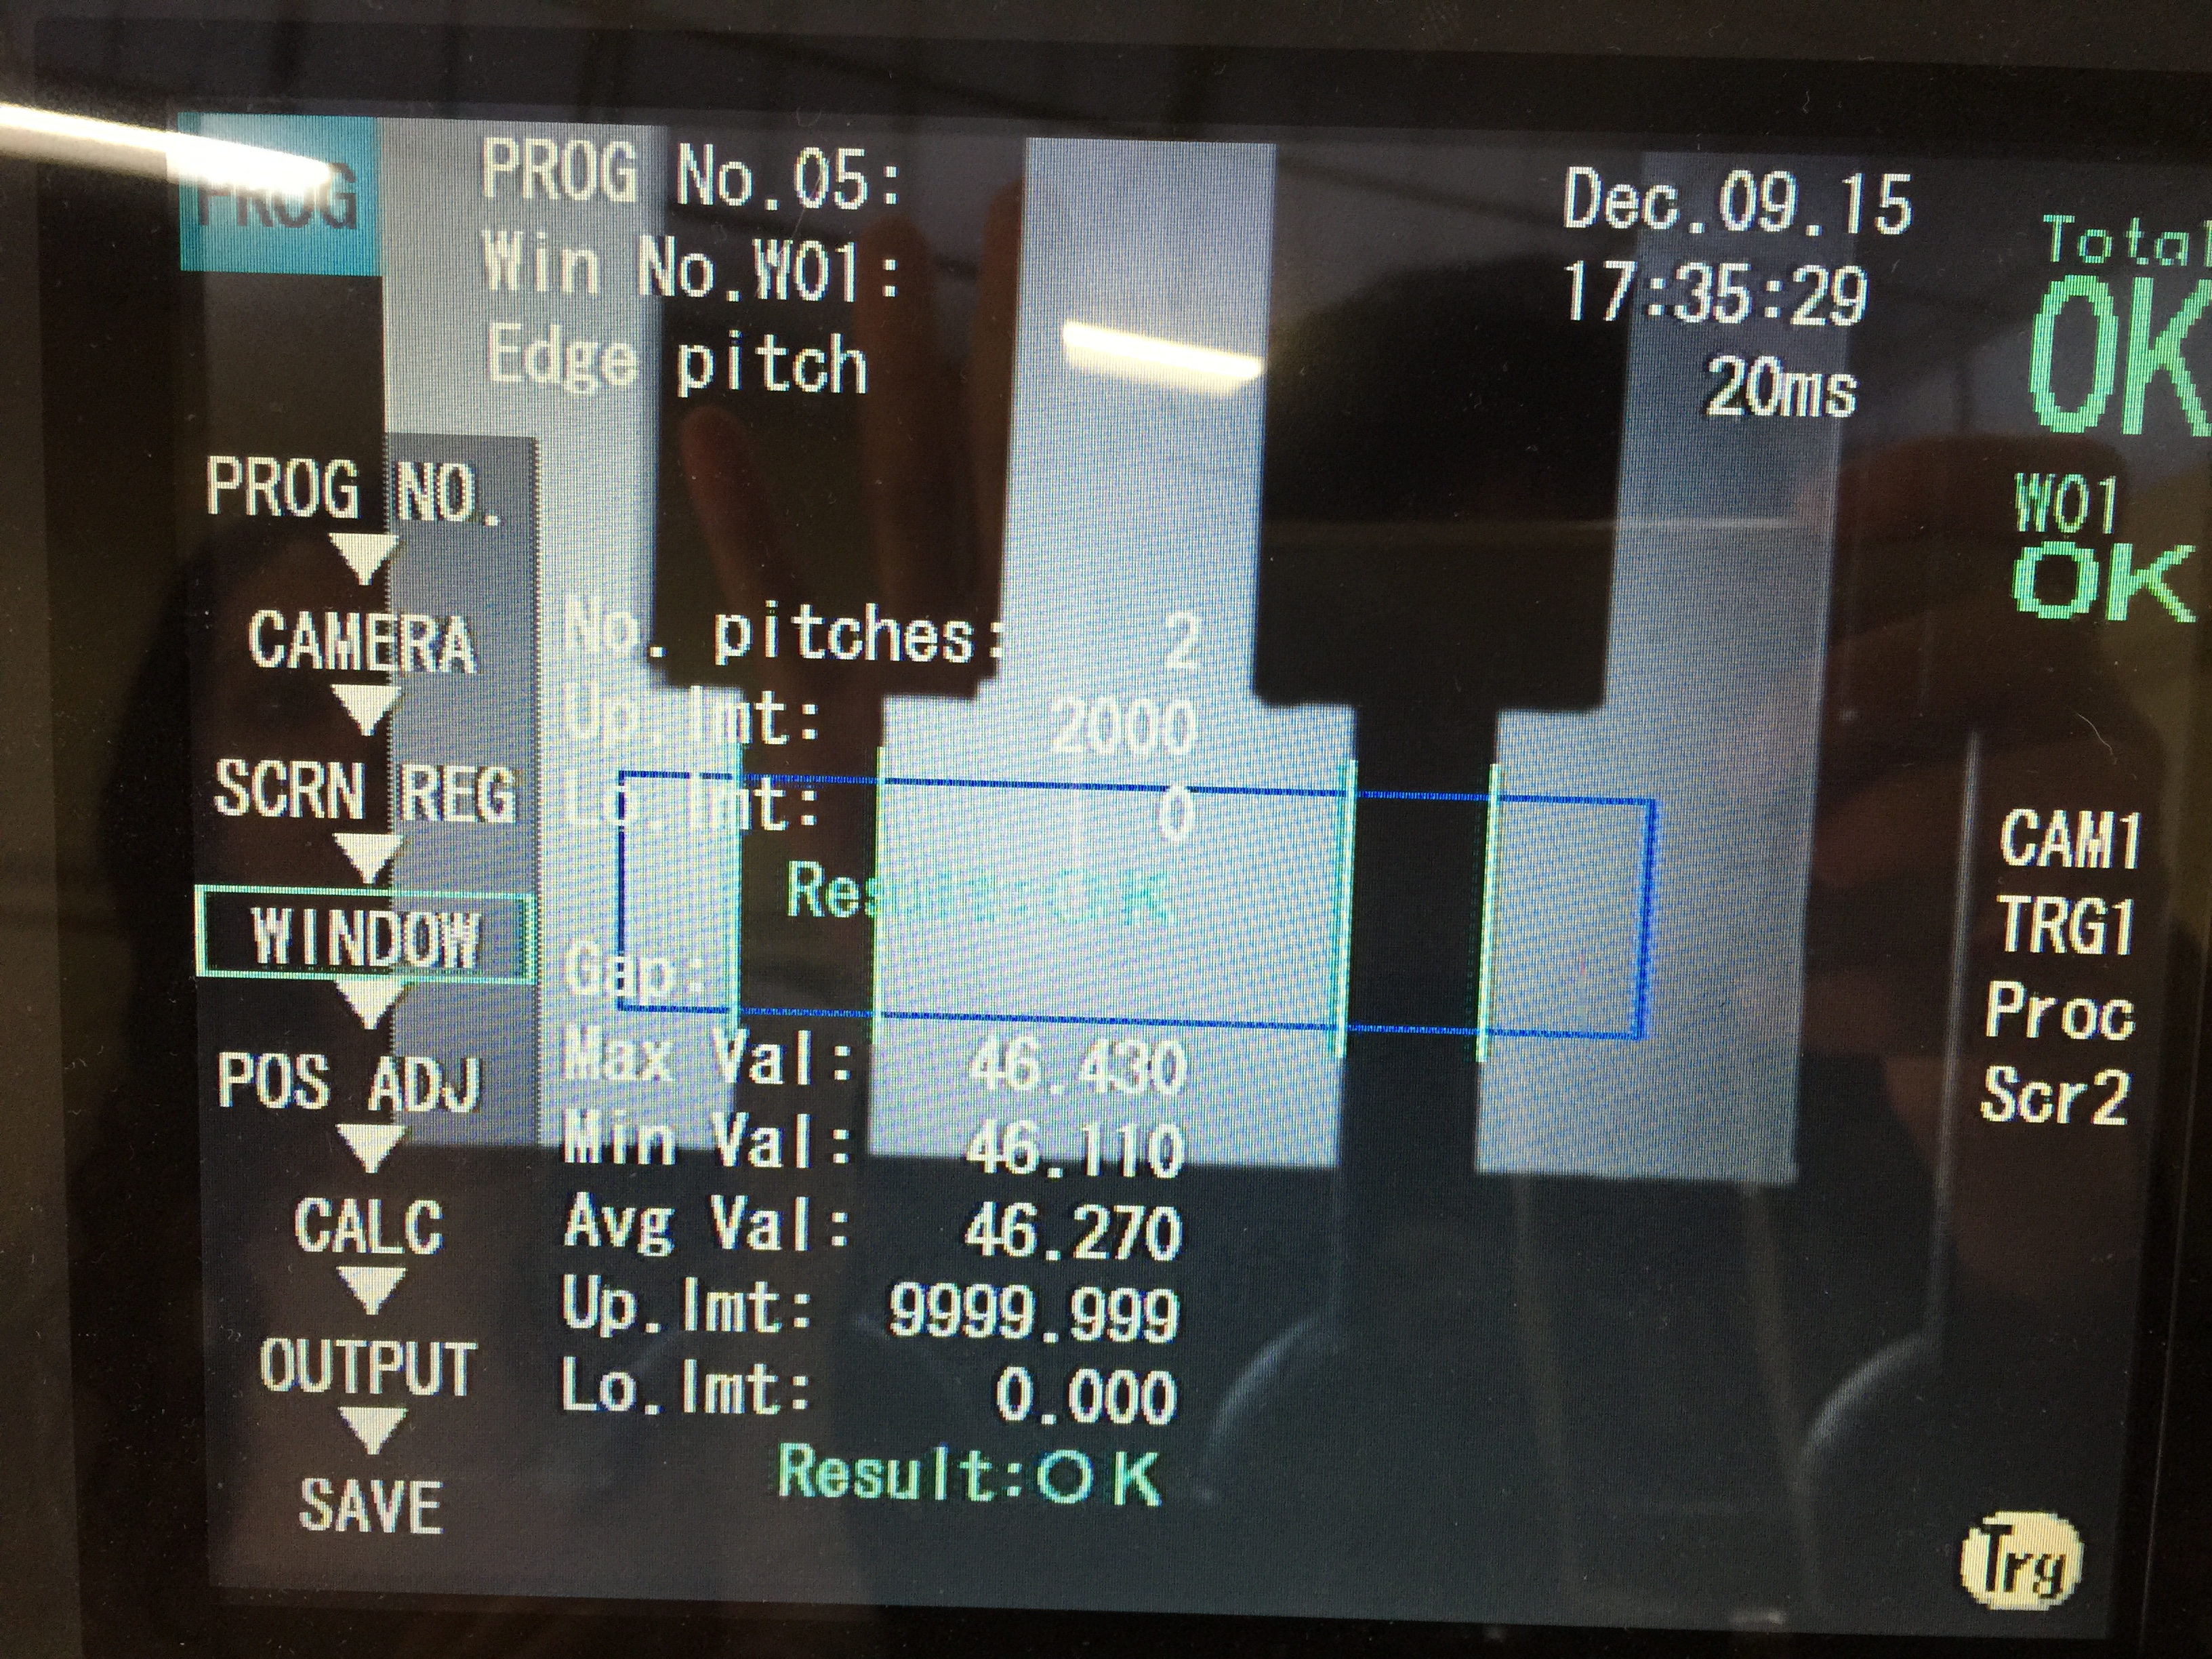
\includegraphics[width=0.6\linewidth]{Pictures/IMG_1224.JPG}
	\caption{Measurement of edge pitch}
	\label{fig:edgepitch2}
\end{figure} 
Here, we can see that both edges are correctly identified and measured.
Because the object stand was move closer to the camera, the measurement value has changed as well.


\section{Caps Detection}
In this part, we try to program to detect perfume caps.
If the system can tell whether the perfume caps are there or not, then we can say it is a successful system for cap detection.\\
\\
First, we set "Measure" to "Multi pattern position".
Second, we manually give a search window in the image so that the detection system can only search the object in the search window (blue triangle in Figure \ref{fig:window}).
Then we set pattern window for perfume cap, which is the white triangle shown in the Figure \ref{fig:window}.

\begin{figure}[H]
	\centering
	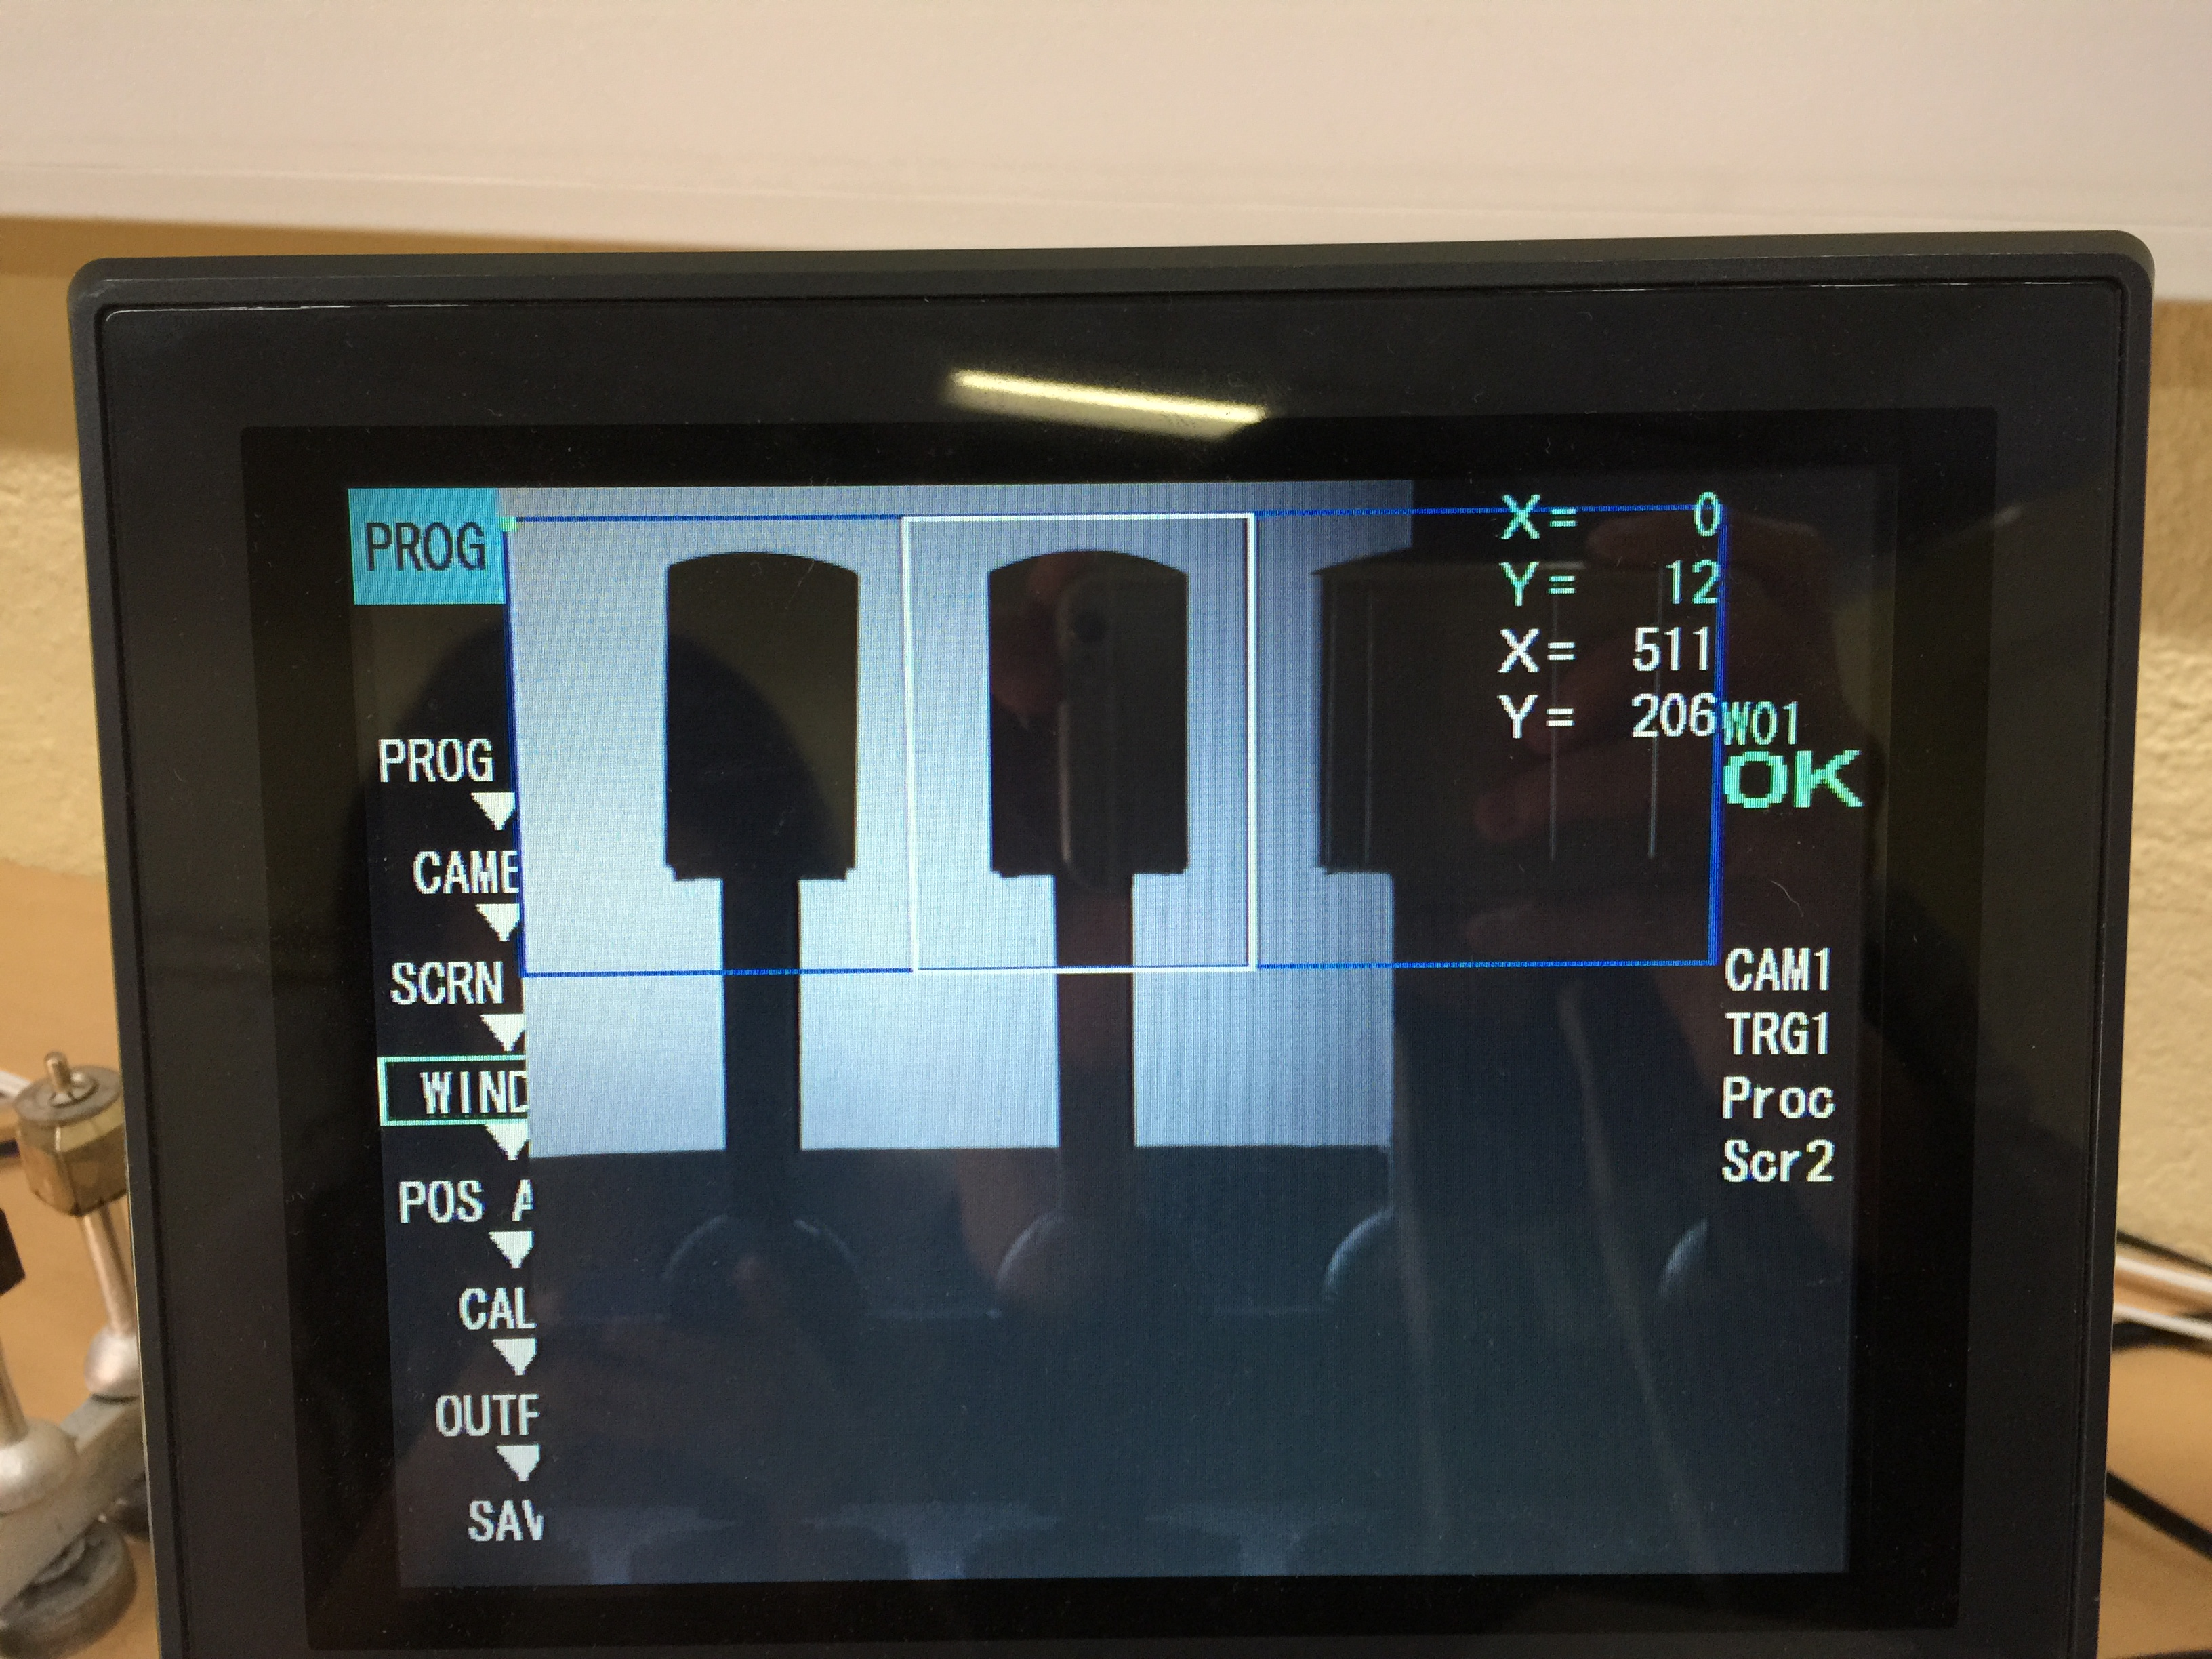
\includegraphics[width=0.6\linewidth]{Pictures/IMG_1225.JPG}
	\caption{Search window (blue) and pattern window (white)}
	\label{fig:window}
\end{figure} 

After setting up all the configuration, we start to use external trigger to grab pictures of outcome of detection (Figure \ref{fig:caps}). In the Figure \ref{fig:capsa}, we are able to see our detection system distinguish two caps in the search window, while in the Figure \ref{fig:capsb}, the system also figure out the cap correctly.\\
\\
In order to check the robustness of the system, we rotate the caps to different angle (Figure \ref{fig:capsc}), and the system can still tell the difference. It turns out the system is robust enough.

\begin{figure}[H]
	\centering
	\subfigure[Two caps]{\label{fig:capsa}
	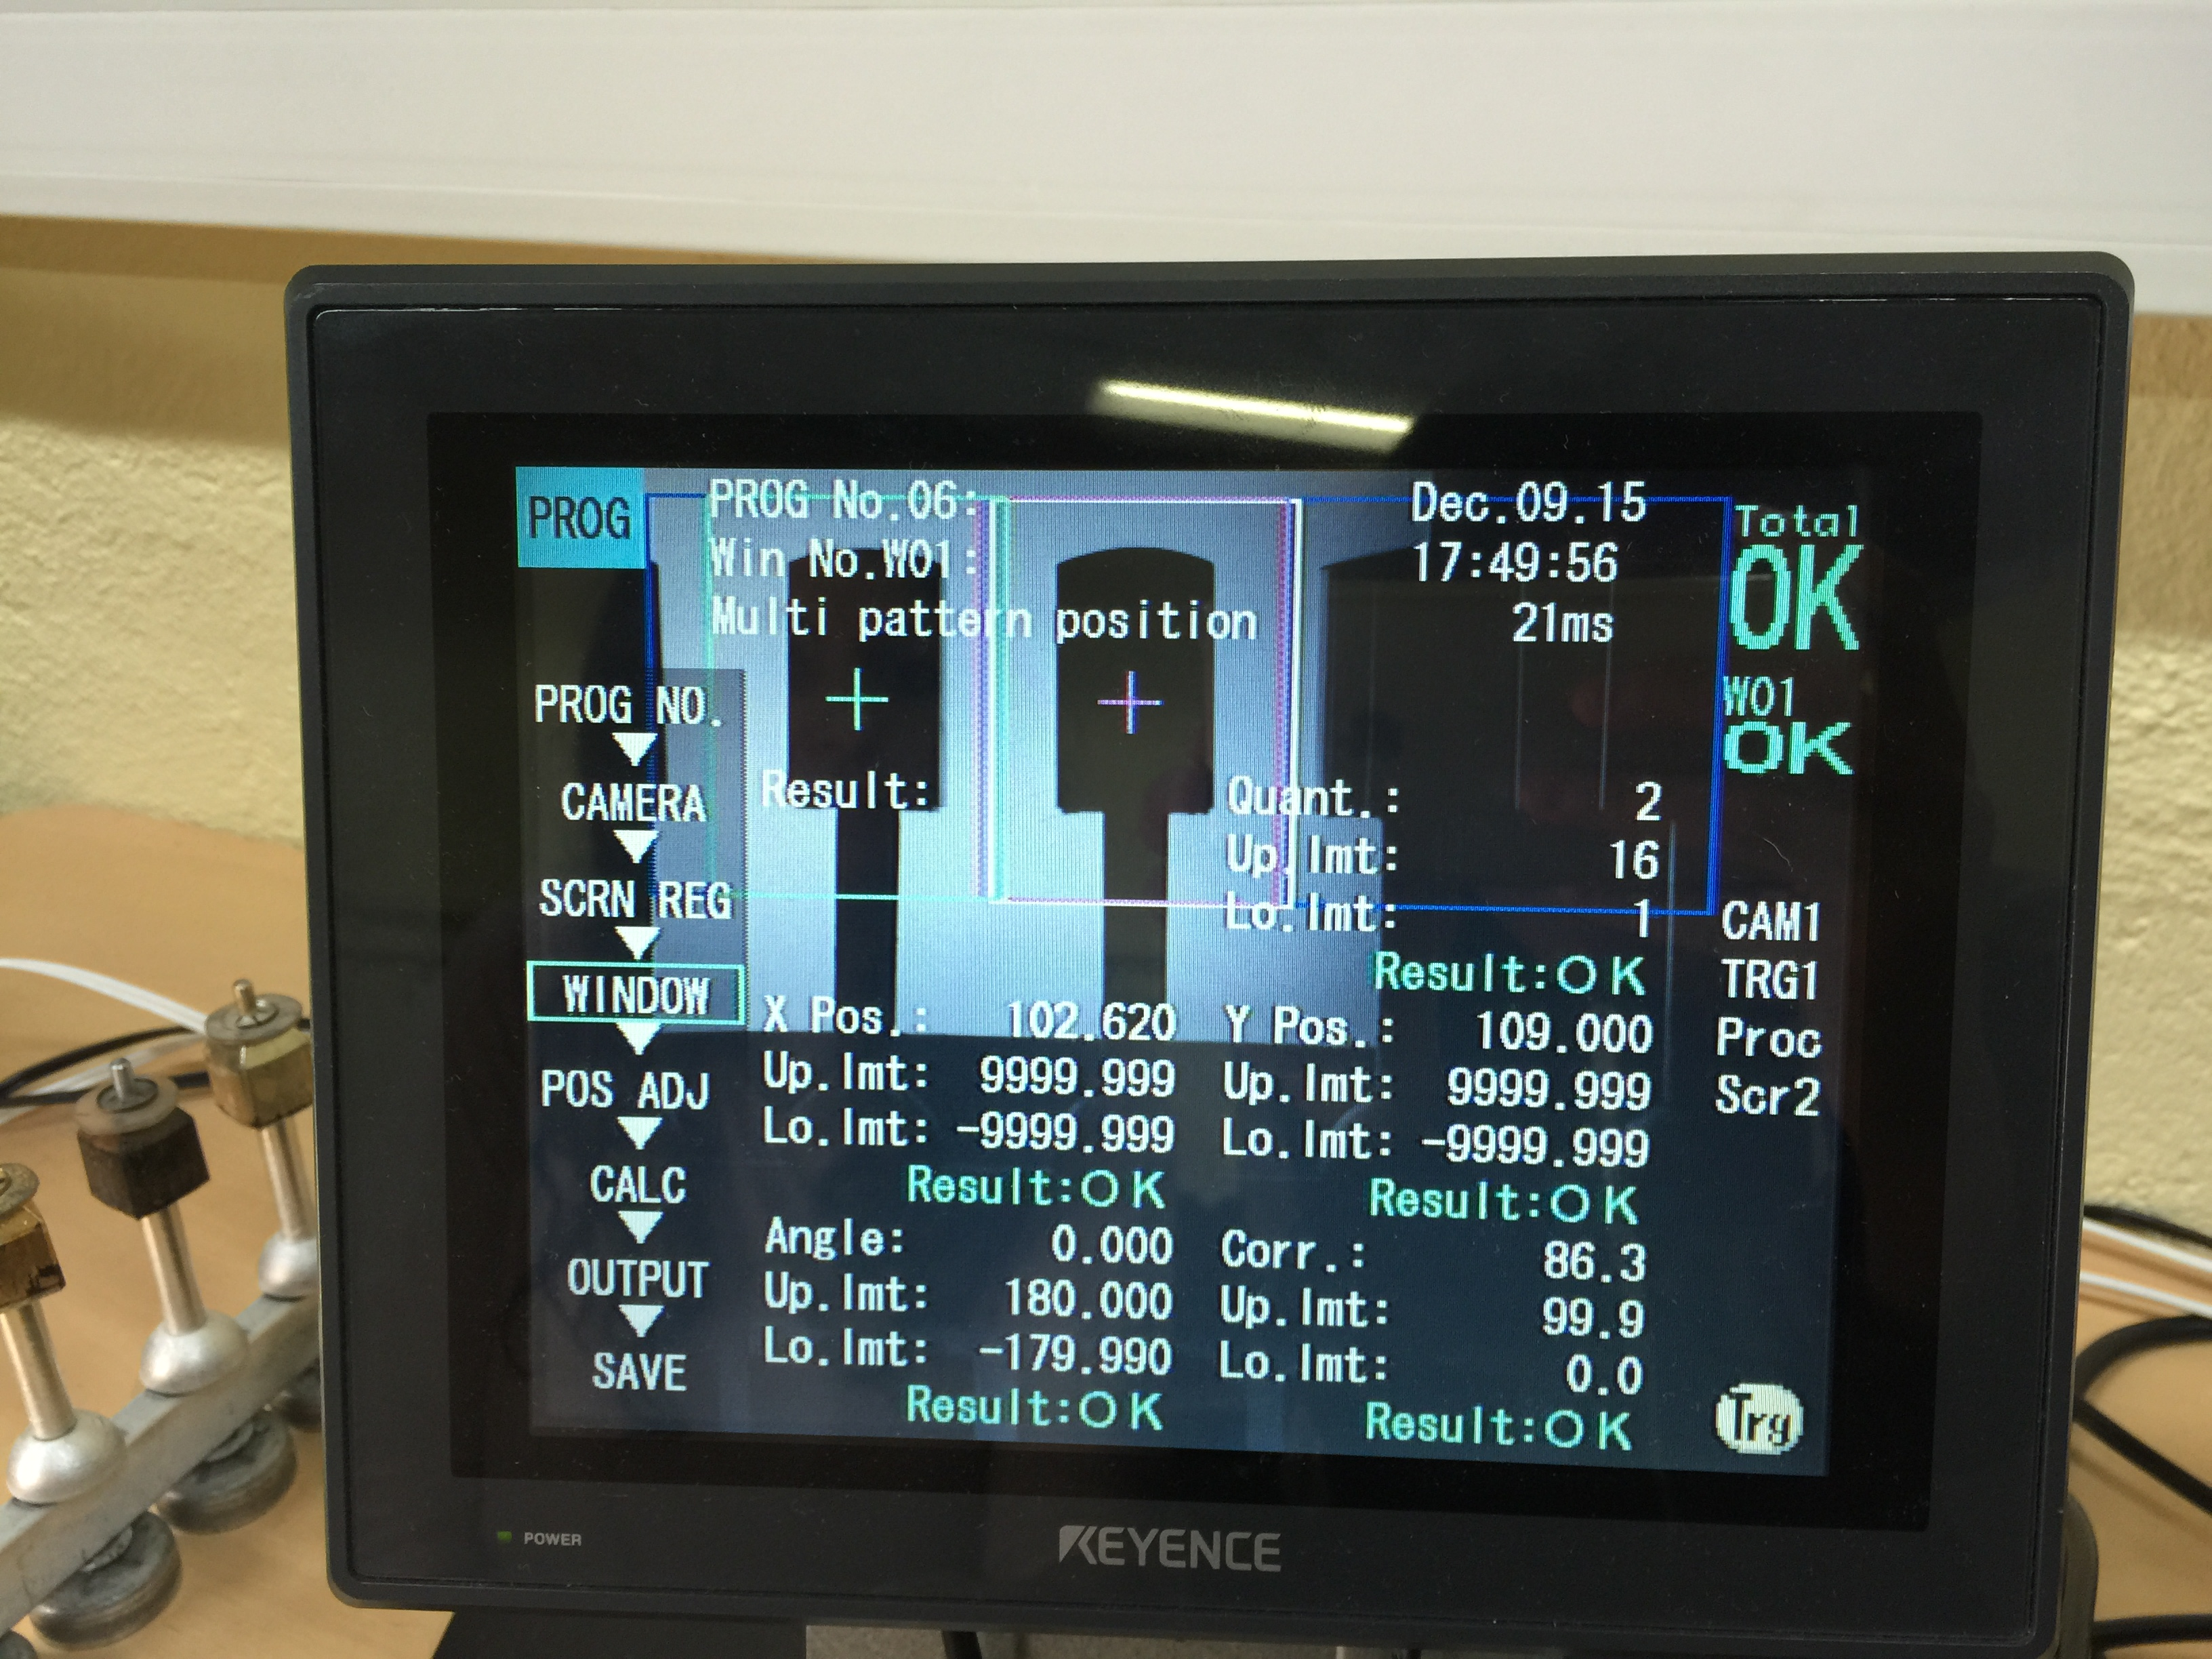
\includegraphics[width=0.6\linewidth]{Pictures/IMG_1226.JPG}
	}
	\subfigure[One caps]{\label{fig:capsb}
	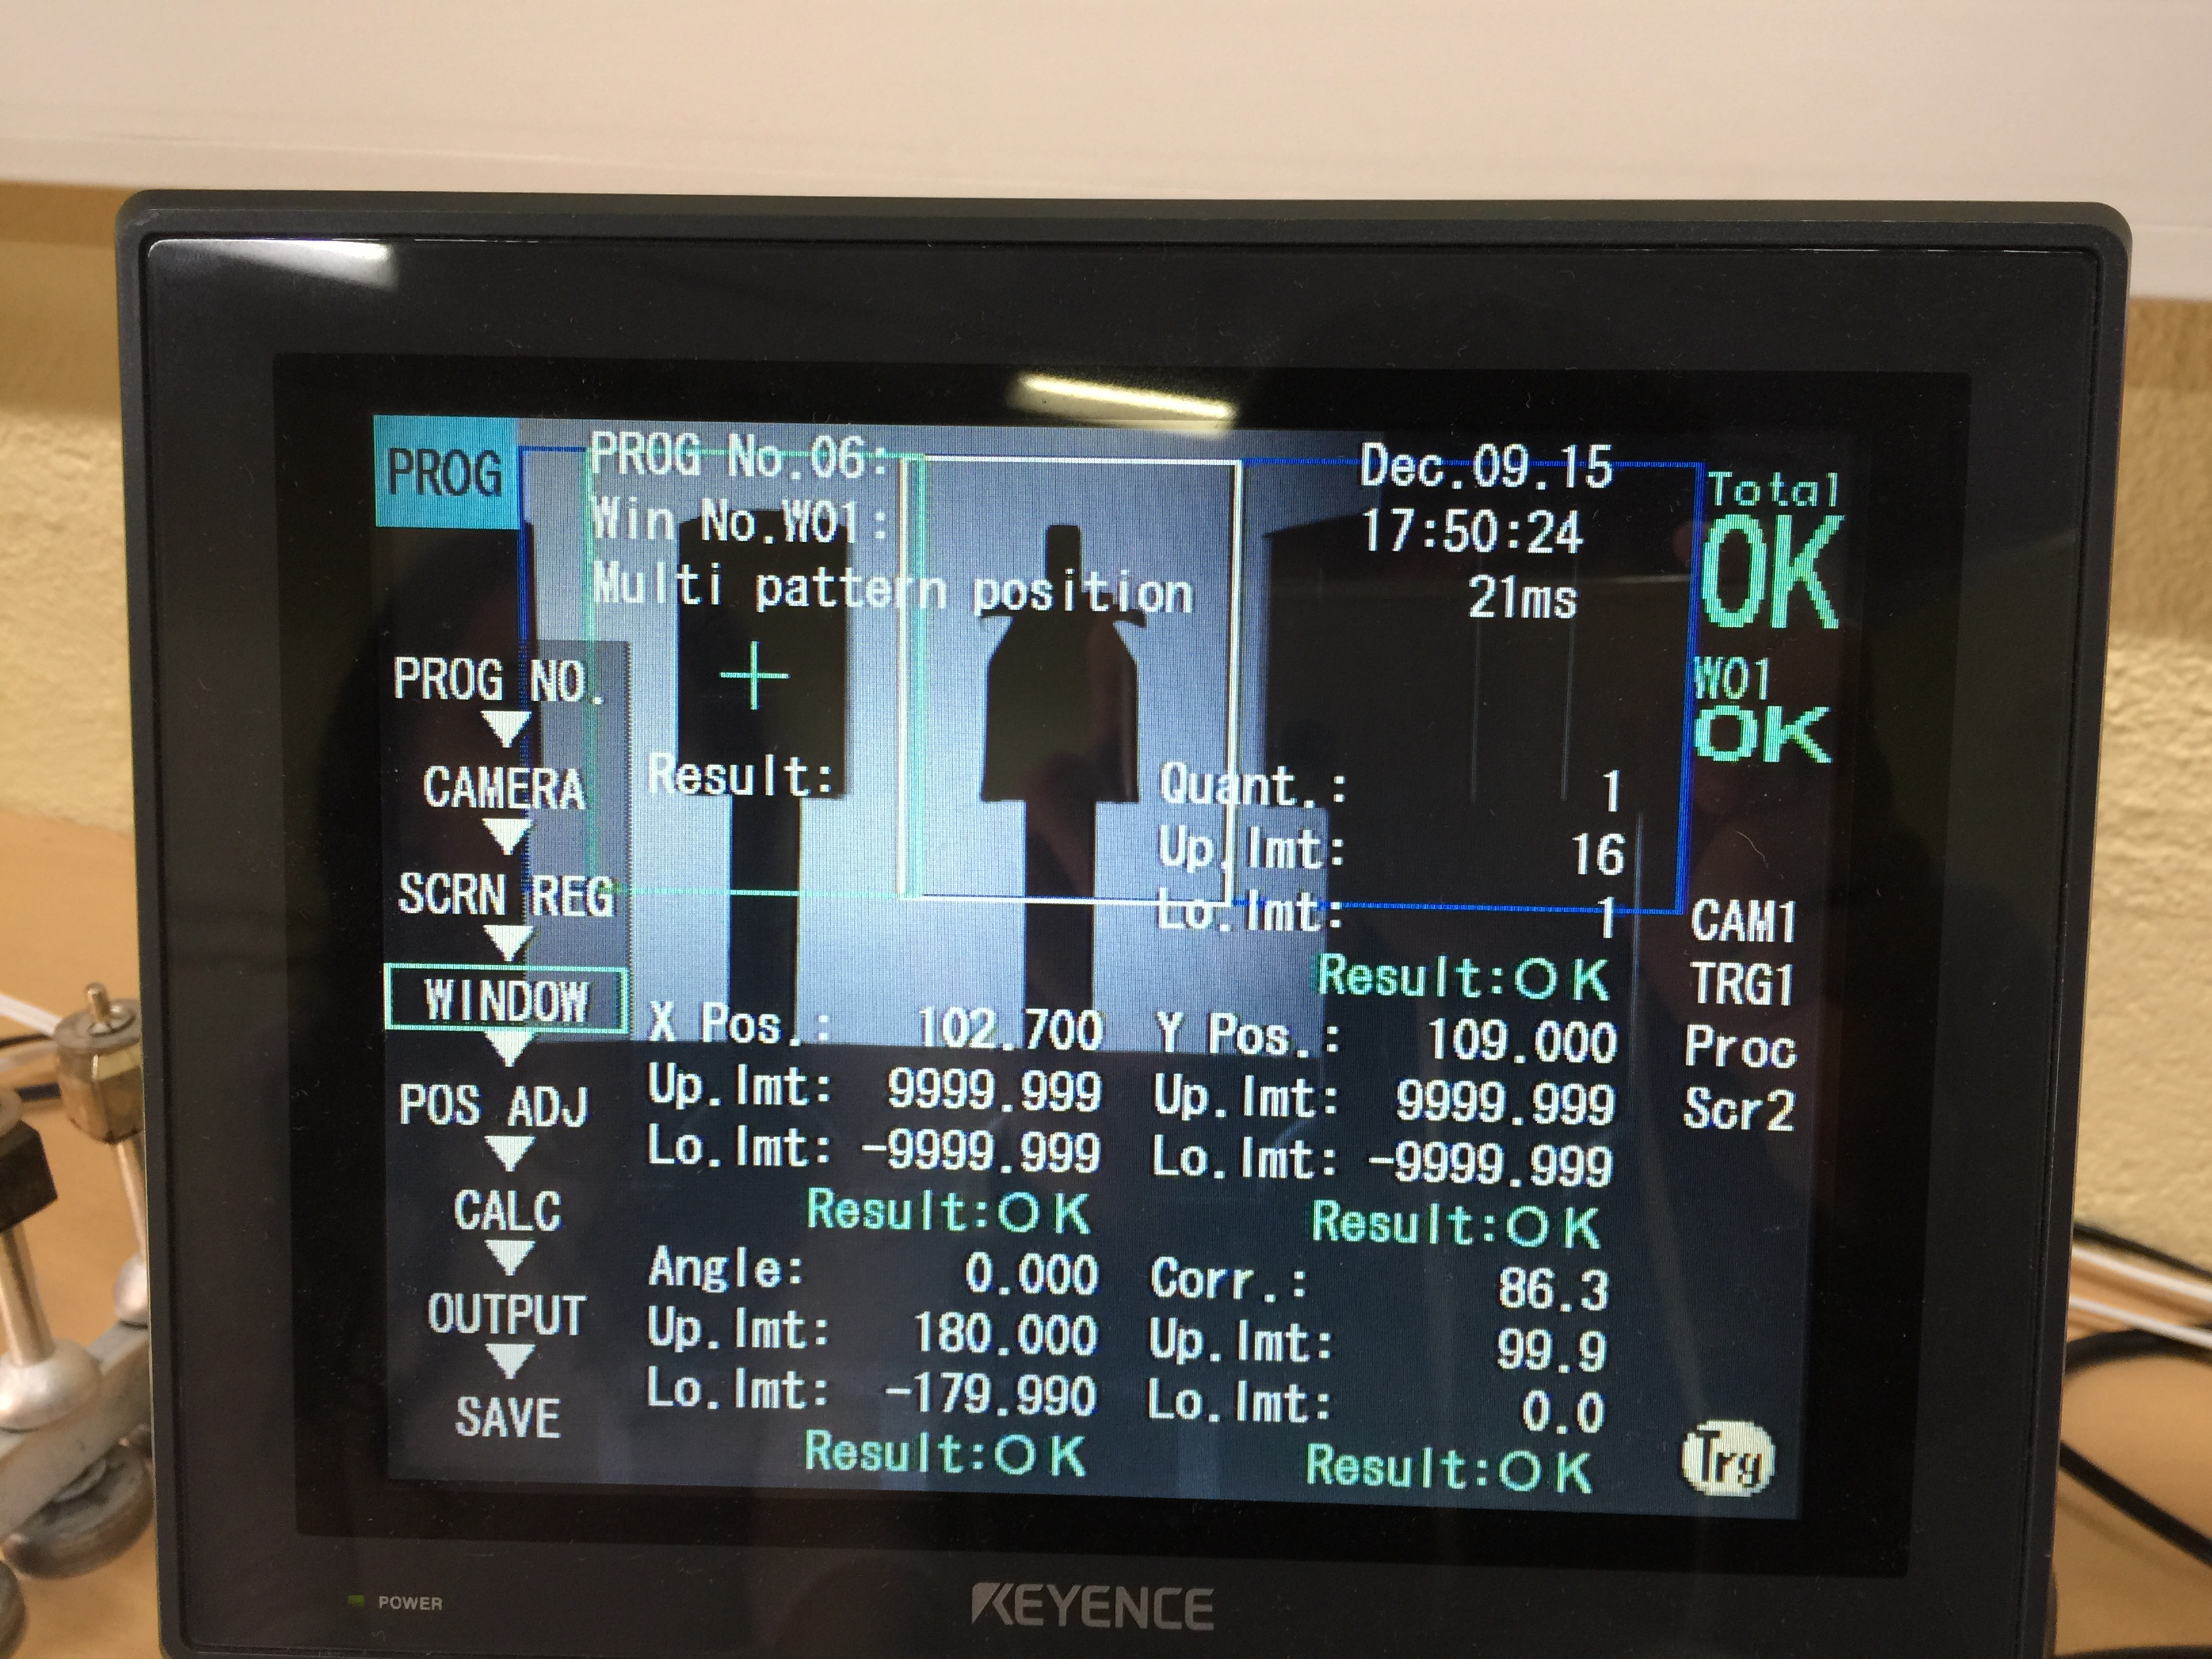
\includegraphics[width=0.6\linewidth]{Pictures/IMG_1227.JPG}
	}
	\subfigure[Rotate caps]{\label{fig:capsc}
	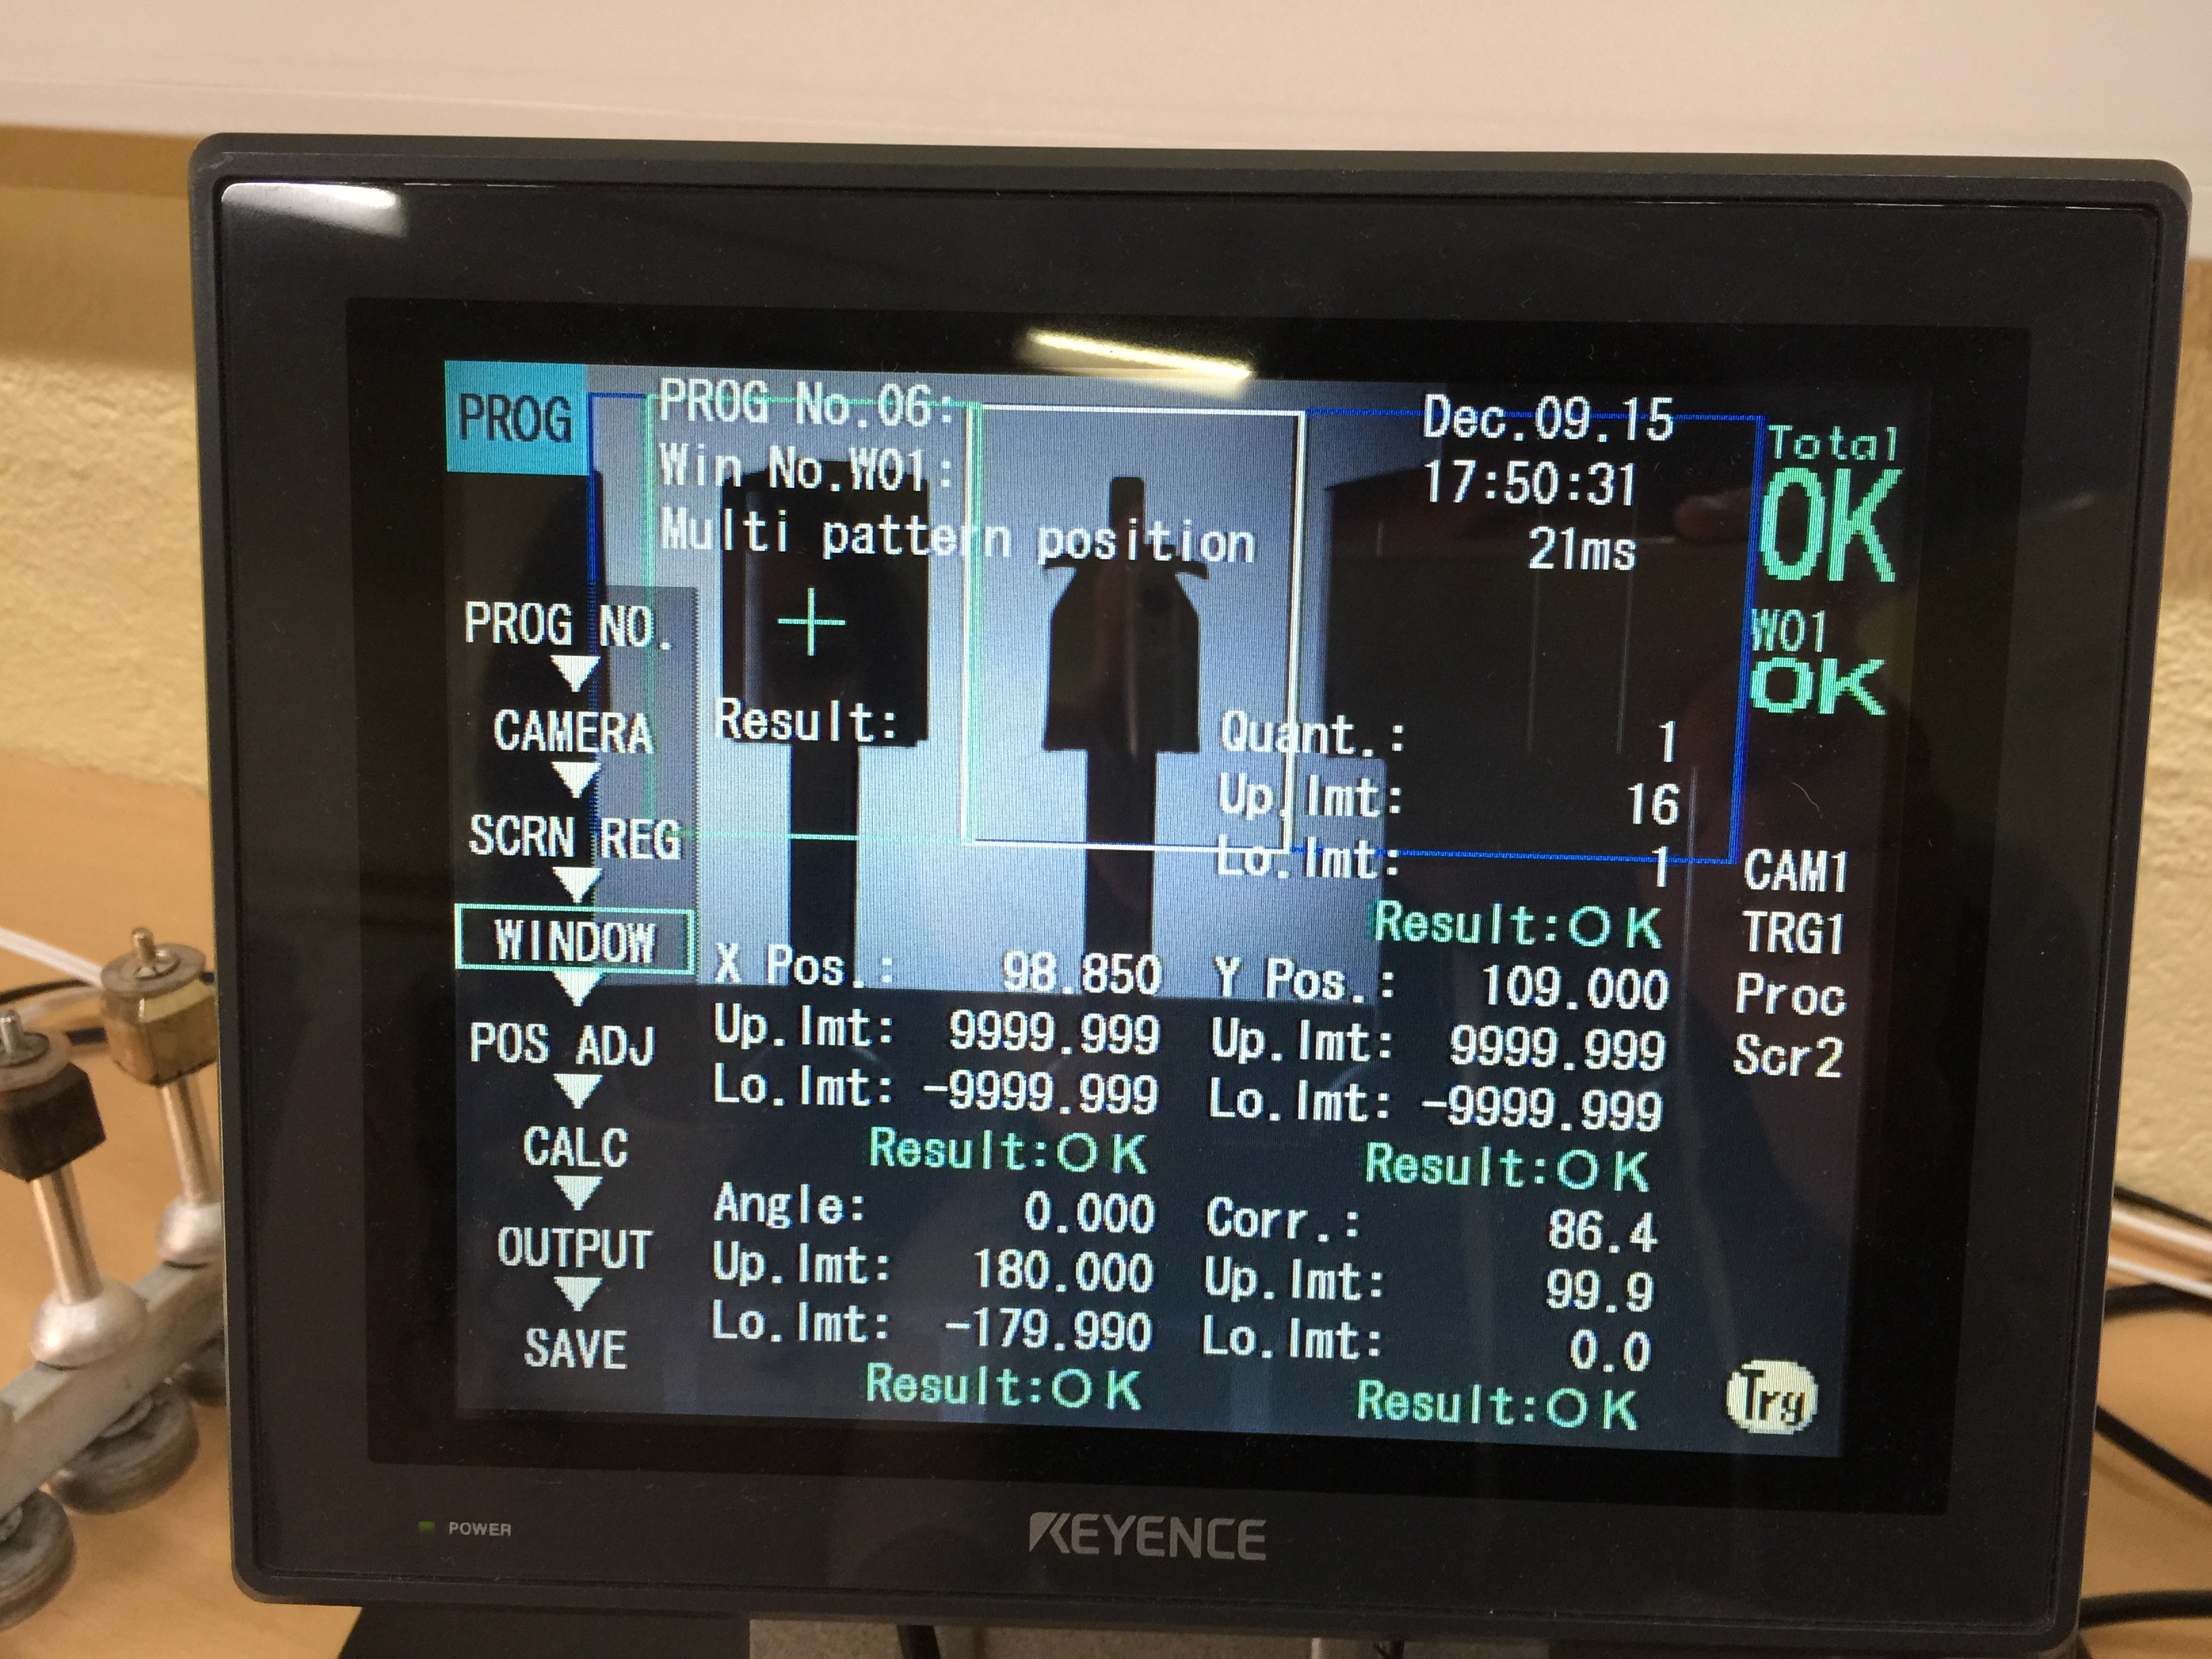
\includegraphics[width=0.6\linewidth]{Pictures/IMG_1228.JPG}
	}
	\caption{Caps detection}
	\label{fig:caps}
\end{figure}

\section{Conclusion}
In this lab, we learn and program a Compact Vision System from KEYENCE. First we program to find the edge of objects and count the number. Second, we select proper tools and  create another detection system to detect whether the perfume caps is in the object.
\section{References}
{[1]} - KEYENCE, General Catalogue. Vision Systems. http://www.mediasrv.co.za/uploads/media/5920.pdf

\end{document}